\section*{Appendix}
\label{sec:appendix}

\subsection*{A. Mathematical Details of the BRAVE Framework}
\label{sec:appendix_math}

\begin{figure*}[!ht]
    \centering
    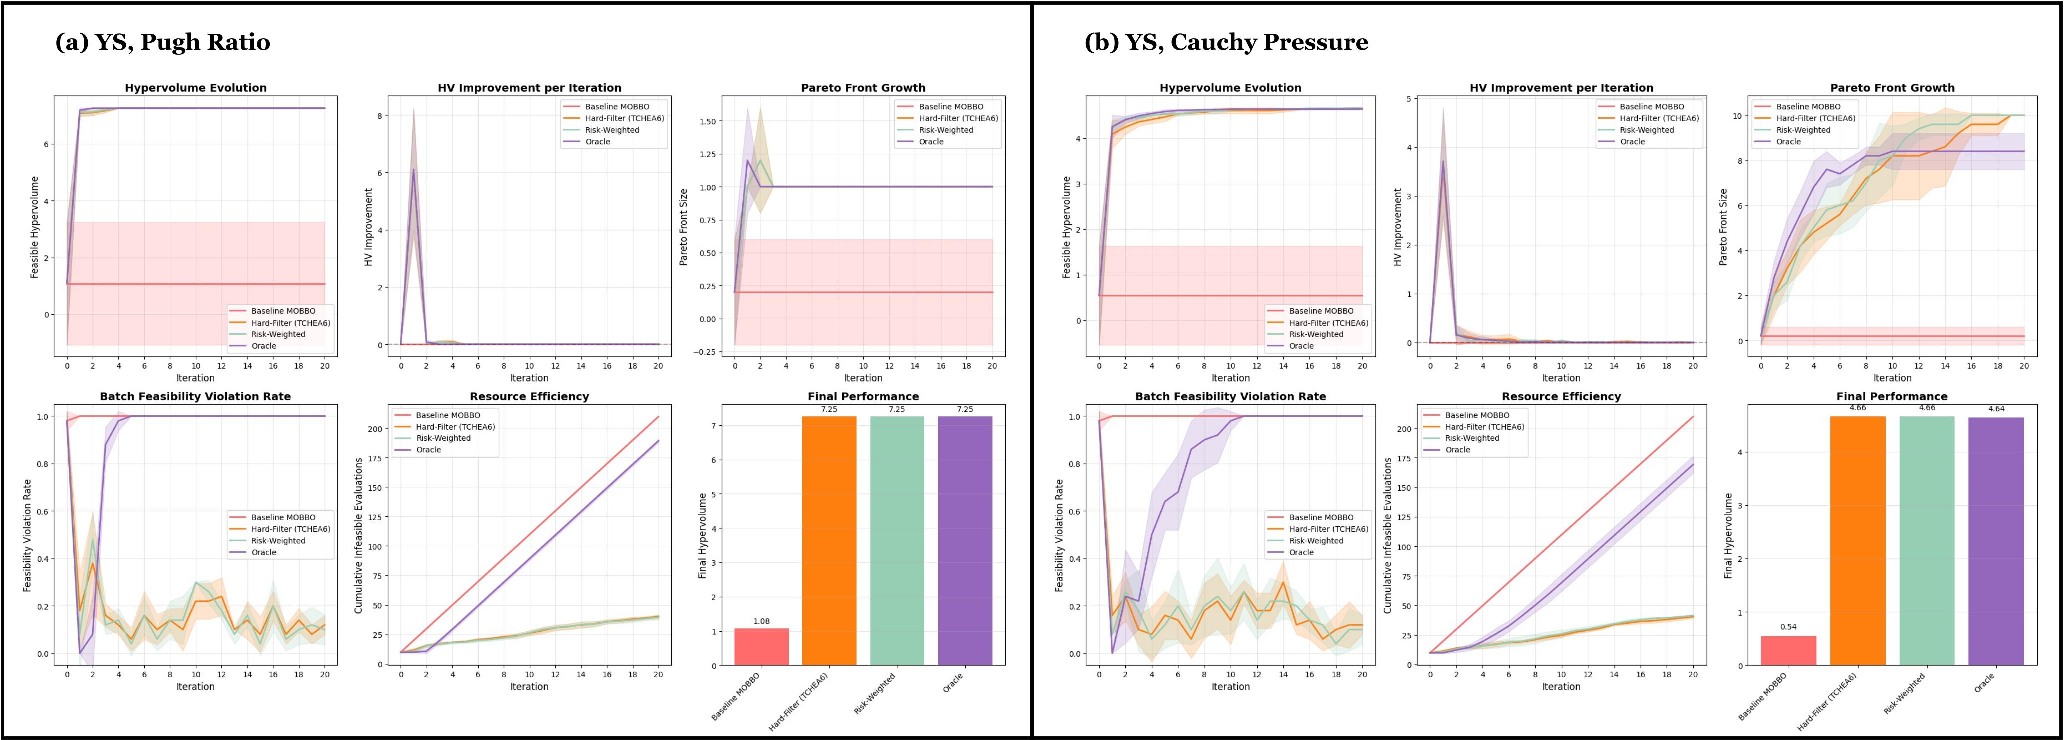
\includegraphics[width=0.95\textwidth]{Sup_figures/benchmark_results.pdf}
    \caption{Benchmarking results for four MOBBO strategies on the six-component HEA system. Two bi-objective tasks are shown: (a) CV(YS)--Pugh ratio and (b) CV(YS)--Cauchy pressure. Metrics: feasible hypervolume (HV), Pareto front size, and feasibility-violation rate (FVR). Risk-weighted MOBBO matches oracle performance while maintaining low FVR.}
    \label{fig:benchmark_results}
\end{figure*}

This section collects the mathematical details of the surrogate modeling, multi-objective acquisition, multi-source fusion, and batch selection components summarized in Section~2.6.

\subsubsection*{A.1 Gaussian Process Regression}

In Bayesian optimization, probabilistic surrogate models are used to represent expensive-to-evaluate objective functions and guide candidate selection through uncertainty-aware predictions. We used Gaussian process regression (GPR) as the surrogate due to its low computational cost and flexible distance-based correlation structure~\cite{Rasmussen:2005:GPM:1162254}.

Assuming there are $N$ previously observed data denoted by $\{\mathbf{X}_{N}, \mathbf{y}_{N}\}$, where $\mathbf{X}_{N} = (\mathbf{x}_{1}, \ldots, \mathbf{x}_{N})$ and $\mathbf{y}_{N} = \left(f(\mathbf{x}_{1}), \ldots, f(\mathbf{x}_{N})\right)$, then the GP probabilistic prediction at unobserved location \textbf{x} is a normal distribution:
\begin{equation}
\label{GP11}
f_{\textrm{GP}}(\mathbf{x}) \mid \mathbf{X}_{N}, \mathbf{y}_{N} \sim \mathcal{N}\left(\mu(\mathbf{x}),\sigma_{\textrm{GP}}^2(\mathbf{x})\right)
\end{equation}
where
\begin{equation}
\begin{aligned}
\label{meancov}
\mu(\mathbf{x}) &= K(\mathbf{X}_{N},\mathbf{x})^\textrm{T}[K(\mathbf{X}_{N},\mathbf{X}_{N})+\sigma^2_{n}I]^{-1} \mathbf{y}_{N}\\
\sigma_{\textrm{GP}}^2 (\mathbf{x})  &=  k(\mathbf{x},\mathbf{x}) - K(\mathbf{X}_{N},\mathbf{x})^\textrm{T} [K(\mathbf{X}_{N},\mathbf{X}_{N})+\sigma^2_{n}I]^{-1}K(\mathbf{X}_{N},\mathbf{x})
\end{aligned}
\end{equation}
here, $k$ is a real-valued kernel function to calculate correlations, $K(\mathbf{X}_{N},\mathbf{X}_{N})$ as a $N \times N$ matrix with $m,n$ entry as $k(\mathbf{x}_{m}, \mathbf{x}_{n})$, and $K(\mathbf{X}_{N}, \mathbf{x})$ is a $N \times 1$ vector with $m^{th}$ entry as $k(\mathbf{x}_{m}, \mathbf{x})$.  The term $\sigma^2_{n}$ is used to model experiment errors. A common choice for kernel function is squared exponential:
\begin{equation}
\label{eq:5}
k(\mathbf{x},\mathbf{x'}) = \sigma_s^2 \exp\left(- \sum_{h = 1}^{d} \frac {(x_h-x'_h)^2}{2l_h^2}\right )
\end{equation}
where $d$ is the dimensionality of the input space, $\sigma_s^2$ is the signal variance, and $l_h$, where $h = 1,2,\ldots,d$, is the characteristic length-scale to determine correlation strength between data points within dimension $h$.

\subsubsection*{A.2 Informative Priors}

Although standard GPR sets the mean function to zero, this forfeits the opportunity to encode prior knowledge. An informative prior instead sets the mean function to a physics-based model prediction, $\mu(\mathbf{x})$, and trains the GPR on the discrepancy $f'(\mathbf{x}) = f_{\textrm{exp}}(\mathbf{x}) - \mu(\mathbf{x})$ between experimental observations and the prior. The posterior $f = f' + \mu$ defaults to the physics-based prediction where no experimental data exist, and overrides it where observations are available.

In this work, we used GPR with an informative prior that integrates physical insights from the Varvenne--Luque--Curtin solid solution strengthening model~\cite{varvenne2016theory} as the prior, $\mu$. This model captures the strengthening behavior of FCC HEAs by accounting for solute misfit volumes, modulus mismatch, and local lattice distortions in a fully random solution. We combined this physics-based prior with limited experimental data, including Vickers hardness (HV) and temperature-dependent yield strength (YS) measurements.

Let the true composition-temperature-dependent mechanical behavior of the HEAs be denoted by $f_{\textrm{exp}}(\mathbf{x})$, where $\mathbf{x}$ is a vector describing the alloy composition and test temperature. The GPR model is built over the residual between experimental observations and the prior prediction, $f_{\textrm{dis}}(\mathbf{x}) = f_{\textrm{exp}}(\mathbf{x}) - \mu(\mathbf{x})$. The final GPR prediction is then:
\[
f(\mathbf{x}) = f_{\textrm{dis}}(\mathbf{x}) + \mu(\mathbf{x}).
\]

The machine learning models were developed using data from~\cite{hastings2025accelerated} in conjunction with the {\tt CBFV}~\cite{Murdock2020IsProperties} and {\tt HEACalculator} packages~\cite{doguhan_sariturk_2022_7429046} for composition feature generation. These tools generated over 5000 features for each composition, which were subsequently optimized using the RecursiveByShapValues method~\cite{Prokhorenkova2018CatBoost:Features} to eliminate redundant features based on SHAP values. Given the tabular nature of the dataset, with a limited number of datapoints and a high dimensionality of features, the CatBoost gradient boosting algorithm~\cite{Prokhorenkova2018CatBoost:Features} was used.

\subsubsection*{A.3 Multi-Objective Optimization via EHVI}

Because EHVI is implemented in minimization form, the four desirable-to-maximize objectives (YS, UTS/YS, strain at UTS, and $H_\text{dyn}/H_\text{qs}$) were sign-inverted before surrogate modeling and hypervolume calculation, while DoP remained in its original minimization form.

A multi-objective optimization problem is defined as
\begin{equation}
\label{eq:problem_app}
    \mbox{minimize}\,\,\,  \{f_1(\textbf{x}), ...,f_n(\textbf{x})\}, \textbf{x} \in \mathcal{X}
\end{equation}
where $f_1(\textbf{x}),\ldots, f_n(\textbf{x})$ are the objectives and $\mathcal{X}$ is the feasible design space. Typically, no single solution simultaneously optimizes all objectives. The solution is instead a set of non-dominated designs with trade-offs, forming the Pareto front in the objective space. The optimal solutions $\mathbf{y}$ are denoted as $\mathbf{y}\prec \mathbf{y'}$ and expressed as
\begin{equation}
\begin{aligned}
   \{\mathbf{y}: \mathbf{y} & = (y_1, y_2, \ldots, y_n), \; y_i \leq y_i' \;\; \forall \; i \in \{1, 2, \ldots, n\}, \\
   &  \exists \; j \in \{1, 2, \ldots, n\} : y_j < y'_j\}
\end{aligned}
\end{equation}
where $\mathbf{y}' = (y_1', y_2', \ldots, y_n')$ denotes any possible objective output.

Several approaches exist for approximating the Pareto front, including weighted sum~\cite{marler2010weighted}, adaptive weighted sum~\cite{kim2005adaptive}, normal boundary intersection~\cite{das1998normal}, and hypervolume indicator methods~\cite{beume2009s,bradstreet2010fast,emmerich2011hypervolume,fonseca2006improved,russo2013quick,yang2007novel,zitzler1999multiobjective}. Hypervolume is the space bounded by a fixed reference point and the current Pareto front approximation; maximizing it pushes the approximation toward the true Pareto front. The acquisition function used here is Expected Hypervolume Improvement (EHVI), computed via the recursive decomposition method of Zhao et al.~\cite{zhao2018fast}. Following~\cite{feliot2017bayesian}, EHVI is defined as
\begin{equation}
    \mathbb{E}[\textrm{{HVI}}({\mathbf{y}})] =\int_U \mathbb{P}(\mathbf{y} \prec{\mathbf{y}'})d{{\mathbf{y}'}}
    \label{Expected_app}
\end{equation}
where $\mathbb{P}(\mathbf{y} \prec \mathbf{y}')$ is the probability that $\mathbf{y}'$ dominates $\mathbf{y}$ and $U$ is the dominated hypervolume. Given an independent GP for each objective, the posterior predictive is $y_i \sim \mathcal{N}(\mu_i , \sigma_i^2)$ where $i\leq m$ and $\mu_i,\sigma_i^2$ are the mean and variance of the $i^{th}$ objective. For a new candidate:
\begin{equation}
    \mathbb{P}(\mathbf{y} \prec \mathbf{y}') = \prod_{i=1}^m \Phi \left ( \frac{y_i' - \mu_i}{\sigma_i} \right )
    \label{prob_app}
\end{equation}
where $\Phi$ is the CDF of the standard normal. Details regarding the closed-form expression of Eq.~(\ref{Expected_app}) can be found in Refs.~\cite{zhao2018fast,feliot2017bayesian,while2011fast,jaszkiewicz2018improved,khatamsaz2020efficient}.

\subsubsection*{A.4 Multi-Source Modeling via Reification}

Four objectives (YS, UTS/YS, strain at UTS, $H_\text{dyn}/H_\text{qs}$) were measured experimentally; the fifth (DoP) was a simulation output derived from FEM models calibrated to the tensile and SHPB data acquired in the same iteration. DoP therefore passed through a two-level model chain---experiment $\rightarrow$ constitutive calibration $\rightarrow$ FEM $\rightarrow$ GP---and its uncertainty compounded surrogate approximation error with upstream calibration error. All five objectives entered the EHVI computation as GP posterior distributions regardless of their origin.

To avoid assumptions about the hierarchy of information sources, we estimated inter-source correlations using the reification technique~\cite{allaire2012fusing,thomison2017model}. Following~\cite{Winkler_1981}, the fused mean and variance are:
\begin{equation}
\label{e:WinklerMeanGen_app}
\mathbb{E} [\hat{f}(\mathbf{x})]=\frac{\mathbf{e}^\textrm{T} \tilde{\Sigma}(\mathbf{x})^{-1}  \boldsymbol{\mu}(\mathbf{x})}{\mathbf{e}^\textrm{T} \tilde{\Sigma}(\mathbf{x})^{-1} \mathbf{e}}
\end{equation}
\begin{equation}
\label{e:WinklerVarianceGen_app}
\textrm{Var}\left(\hat{f}(\mathbf{x})\right) = \frac{1}{\mathbf{e}^\textrm{T} \tilde{\Sigma}(\mathbf{x})^{-1} \mathbf{e}}
\end{equation}
where $\mathbf{e} = [1,\ldots,1]^\textrm{T}$, $\boldsymbol{\mu}(\mathbf{x}) = [\mu_1(\mathbf{x}),\ldots,\mu_m(\mathbf{x})]^\textrm{T}$ given $m$ information sources, and $\tilde{\Sigma}(\mathbf{x})$ is the covariance matrix with diagonal elements $\sigma_i^2$ and off-diagonal elements $\bar{\rho}_{ij} \sigma_i \sigma_j$. The correlation coefficient $\bar{\rho}_{ij}$ is calculated via reification:
\begin{equation}
\bar{\rho}_{ij}(\mathbf{x}) = \frac{\sigma_j^2(\mathbf{x})}{\sigma_i^2(\mathbf{x}) + \sigma_j^2(\mathbf{x})} \rho_{ij}(\mathbf{x}) + \frac{\sigma_i^2(\mathbf{x})}{\sigma_i^2(\mathbf{x})+\sigma_j^2(\mathbf{x})} \rho_{ji}(\mathbf{x})
\label{e:VWrho_app}
\end{equation}
where
\begin{equation}
\begin{aligned}
\rho_{ij}(\mathbf{x}) &= \frac{\sigma_i(\mathbf{x})}{\sqrt{\left(\mu_i(\mathbf{x})-\mu_j(\mathbf{x})\right)^2 + \sigma_i^2(\mathbf{x})}}, \\
\rho_{ji}(\mathbf{x}) &= \frac{\sigma_j(\mathbf{x})}{\sqrt{\left(\mu_i(\mathbf{x})-\mu_j(\mathbf{x})\right)^2 + \sigma_j^2(\mathbf{x})}}.
\end{aligned}
\label{e:rho_app}
\end{equation}

\subsubsection*{A.5 Batch Bayesian Optimization}

GP surrogates depend on kernel length-scale hyperparameters that control correlation strength across the input space. Although standard tuning methods (e.g., maximum likelihood~\cite{Rasmussen:2005:GPM:1162254}, cross-validation) are effective with sufficient data, they can become trapped in local optima when training data are sparse~\cite{joy2020batch,couperthwaite2020materials}.

To address this, we constructed a large ensemble of GPs with randomly sampled length-scales, each encoding a different smoothness assumption~\cite{joy2020batch}. Each GP made a different inference about the underlying objective function, yielding different candidate suggestions:
\begin{equation}
    \textbf{x}_{1:n} = \arg\max_{\mathbf{x} \in \chi}  \textrm{EHVI}^{N}(\textbf{x} | \textrm{GP}(\mathbb{D}_N,\theta_{1:n}))
\end{equation}
where $n$ Gaussian processes were built with different hyperparameter sets $\theta$ given data $\mathbb{D}$. From the $n$ candidate suggestions, k-medoids clustering selected a batch of compositions that maximized diversity while preserving aggregate hypervolume gain.

\subsection*{B. Benchmarking Risk-Aware Multi-Objective Bayesian Optimization}
\label{sec:appendix_benchmark}

To quantitatively assess the effectiveness of the proposed risk-aware multi-objective Bayesian optimization (MOBBO) strategy, we constructed a controlled computational benchmark based on the six-component Al--V--Cr--Fe--Co--Ni HEA space. The full design space was discretized at 4~at.\% resolution, generating a pool of 23{,}694 distinct compositions with precomputed objective properties and phase stability metrics.

Two bi-objective optimization problems were defined:
(i) maximize yield strength proxy (CV\_YS) and Pugh ratio ($B/G$), and
(ii) maximize CV\_YS and Cauchy pressure ($C_{12} - C_{44}$).
CV\_YS was computed using the Curtin--Varvenne solid solution strengthening model~\cite{varvenne2016theory}; Pugh ratio and Cauchy pressure were approximated via rule-of-mixtures aggregation of elemental elastic constants.

Feasibility was introduced through a dual-database configuration that mimics realistic model discrepancy: screening used TCHEA6 (FCC $\geq 0.99$ at 700$^\circ$C), while ground-truth feasibility labels were assigned from TCHEA7. Any composition with TCHEA7 FCC fraction $<0.99$ was treated as infeasible.

Four acquisition strategies were compared:

\begin{enumerate}
    \item \textbf{Baseline MOBBO}: EHVI applied across the full design space without feasibility awareness.
    \item \textbf{Hard-Filter MOBBO}: EHVI restricted to TCHEA6-predicted FCC-stable compositions.
    \item \textbf{Risk-Weighted MOBBO}: EHVI multiplied by $p_{\text{feas}} = (\text{FCC}_{\text{TCHEA7}})^{\alpha}$ with $\alpha = 2$.
    \item \textbf{Oracle MOBBO}: EHVI weighted by the true binary feasibility label from TCHEA7 (upper bound).
\end{enumerate}

Each campaign selected 10 initial compositions via $k$-medoids clustering, then ran 20 sequential iterations of batch size 10, with GP regressors for objectives and a Random Forest classifier for feasibility. Five random seeds yielded 100 total campaigns per objective pair. Performance was evaluated using feasible hypervolume (HV), Pareto front size, and feasibility violation rate (FVR).

\autoref{fig:benchmark_results} summarizes the results. The differences between strategies are consistent across both objective pairs:



\begin{itemize}

\item \textbf{Baseline MOBBO} fails completely: near-zero feasible HV, trivial Pareto sets, FVR $\approx 1.0$, with $>$90\% of evaluations wasted on infeasible candidates.

\item \textbf{Hard-Filter MOBBO} improves feasibility (FVR $\approx 0.15$) but plateaus early when TCHEA6 mispredictions over-restrict exploration. It achieves HV = 7.25 (Pugh) and 4.66 (Cauchy) but lacks robustness near misclassified boundaries.

\item \textbf{Risk-Weighted MOBBO} matches the oracle in final HV (7.25 and 4.66), maintains low FVR ($\approx 0.15$--0.20), and converges within 3--5 iterations. By penalizing rather than excluding uncertain candidates, it preserves exploration flexibility near critical boundaries.

\item \textbf{Oracle MOBBO} achieves identical final HV but wastes $\approx$170--190 evaluations on infeasible candidates early on, demonstrating that feasibility knowledge alone is insufficient---it must be incorporated into the acquisition function.

\end{itemize}

The oracle result is instructive: perfect feasibility knowledge does not prevent waste. The oracle still aggressively queries high-objective infeasible regions early on ($\approx$170--190 wasted evaluations), because feasibility labels alone do not suppress the acquisition function's attraction to unexplored regions with high predicted performance. Risk-weighted MOBBO avoids this by embedding feasibility directly into the acquisition score, achieving identical final HV with ${\sim}5\times$ fewer wasted evaluations. The lesson parallels the experimental campaign: identifying the feasibility boundary is necessary but not sufficient---the acquisition function must be designed to navigate it.
